% Drawing 154/01-5 -- folder 154, batch 01, archive page 12 (PDF page 13).
% Transcription: figure en tête de la colonne de droite : un faisceau de droites orange (et grises) issues d'un point $s$, coupant une droite jaune en $r$ et $t$ ; les lettres $A$ et $B$ marquent les deux grands triangles de part et d'autre
% Kind: pencil of pseudolines on a line. Method 2 (schematic redraw from the facsimile). Status: ok.
% Notes: Head of the right column: four orange lines through s (and two grey pencil lines) cut the yellow line, the outer two at r and t; A and B mark the two large triangles on either side, in ink above the line and in pencil below. The five small figures at the head of the left column belong to the page but are not covered by this mark (the transcription does not describe them).
% Coordinates: 1 unit = 1 mm = 1/100 of the crop width (bbox in page fractions: [0.52, 0.069, 0.819, 0.162]).
% Redrawn by Claude (claude-opus-5-5), issue #73, 2026-11-07; not checked by a human; not compiled (no TeX in the session).
% Rights: reproduces part of the work -- behind RENDER_TRANSCRIPTS, never published by itself.
\documentclass[tikz,border=3pt]{standalone}
\usepackage{amsmath,amssymb}
\usetikzlibrary{patterns,arrows.meta}
\tikzset{Or/.style={orange!90!black}, Ye/.style={yellow!80!orange}, Lg/.style={green!60!black!70}, Dg/.style={green!45!black}, Br/.style={brown!80!black}, Rd/.style={red!85!black}, Bl/.style={blue!70!black}, Gy/.style={black!40}, pencil/.style={black!45}, struck/.style={black!35}, mark/.style={circle,draw,inner sep=1.3pt}, pt/.style={circle,fill,inner sep=0.9pt}, opt/.style={circle,draw,fill=white,inner sep=1.1pt}}
\begin{document}
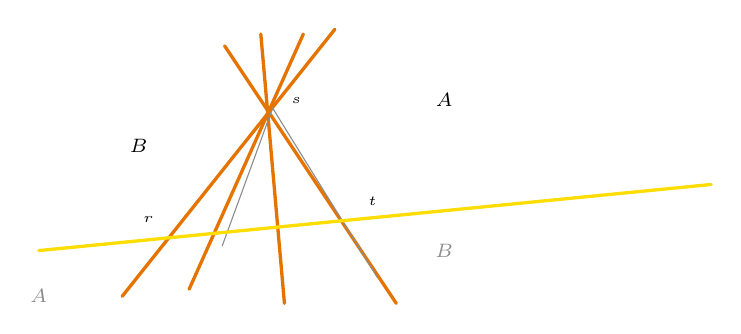
\begin{tikzpicture}[x=1mm,y=1mm,line cap=round,line join=round,font=\scriptsize]
\draw[Or,very thick] (18.5,-39.7) -- (45.5,-5.8);
\draw[Or,very thick] (27,-38.8) -- (41.5,-6.4);
\draw[Or,very thick] (39.1,-40.6) -- (36.1,-6.4);
\draw[Or,very thick] (53.3,-40.6) -- (31.5,-7.9);
\draw[pencil] (37.6,-15.8) -- (31.2,-33.3);
\draw[pencil] (37.6,-15.8) -- (50.9,-37.3);
\draw[Ye,very thick] (7.9,-33.9) -- (93.3,-25.5);
\node[inner sep=1pt] at (40.6,-14.8) {\tiny $s$};
\node[inner sep=1pt] at (21.8,-30) {\tiny $r$};
\node[inner sep=1pt] at (50.3,-27.6) {\tiny $t$};
\node[inner sep=1pt] at (20.6,-20.6) {\scriptsize $B$};
\node[inner sep=1pt] at (59.4,-14.8) {\scriptsize $A$};
\node[inner sep=1pt,pencil] at (7.9,-39.7) {\scriptsize $A$};
\node[inner sep=1pt,pencil] at (59.4,-33.9) {\scriptsize $B$};
\end{tikzpicture}
\end{document}
